\section{Acompanhar Lançamentos}

Este caso de uso tem como função permitir que o usuário consiga acompanhar os lançamentos realizados em sua conta.

\subsection{Caso de uso descritivo}

\begin{table}[h]
  \centering
  \begin{tabular}{|p{4cm} | p{10cm} |}
      \hline
      \small{\textbf{Requisitos Não Funcionais Associados}}	&	Tempo de acesso, segurança, interface amigável e acessível	\\ \hline
      \small{\textbf{Pré-condição}}	&	O usuário deve ser cliente do banco e deve possuir uma conta ativa	\\ \hline
      \small{\textbf{Pós-condição}}	&	O usuário visualiza os lançamentos realizados de acordo com o filtro aplicado	\\ \hline
    \end{tabular}
 \captionof{table}{Condições para o caso de uso Acompanhar Lançamentos}
\end{table}

\textbf{Fluxo de eventos principal:}

\begin{enumerate}
  \item O usuário acessa o sistema utilizando suas credenciais.
  \item O sistema realiza a validação dos dados informados.
  \item O usuário seleciona a opção ``Lançamentos da minha conta''.
  \item O sistema exibe opções de filtros a serem aplicados nos lançamentos.
  \item O usuário seleciona a opção ``Todos os lançamentos''.
  \item O sistema solicita o levantamento dos lançamentos da conta do usuário.
  \item Ao obter os dados dos lançamentos da conta do usuário, o sistema retorna os lançamentos para a tela, informando os lançamentos de acordo com o filtro aplicado.
\end{enumerate}

\textbf{Fluxos secundários:}

\begin{itemize}
  \item \textbf{Fluxo secundário – Acompanhar lançamentos no modo débito}

  No passo 5 do fluxo de eventos principal:
  \subitem Se o usuário selecionar ``Lançamentos no modo débito'', só serão exibidos os lançamentos referentes ao modo débito.

  \item \textbf{Fluxo secundário – Acompanhar lançamentos no modo crédito}

  No passo 5 do fluxo de eventos principal:
  \subitem Se o usuário selecionar ``Lançamentos no modo débito'', só serão exibidos os lançamentos referentes ao modo crédito.
\end{itemize}

\subsection{Diagrama de caso de uso}

O diagrama para o caso de uso Acompanhar Lançamento pode ser visualizado na Figura \ref{cdu:acompanharLancamento}.

\begin{figure}[!htb]
     \centering
     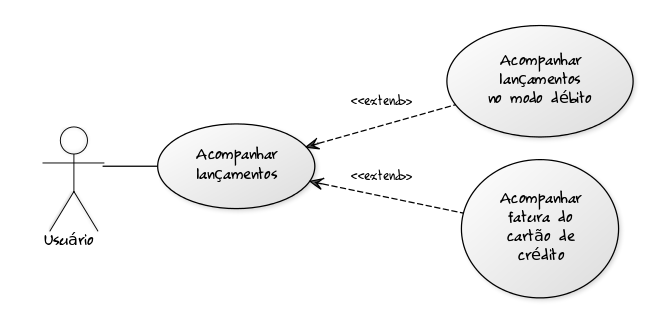
\includegraphics[scale=0.6]{diagramas/caso-de-uso/imagens/acompanharLancamento.png}
     \caption{Caso de uso Acompanhar Lançamento}
     \label{cdu:acompanharLancamento}
\end{figure}

\subsection{Diagrama de classes para o caso de uso}

O diagrama de classes para o caso de uso Acompanhar lançamentos pode ser visualizado na Figura \ref{ddc:acompanharLancamentos}.

\begin{figure}[!htb]
     \centering
     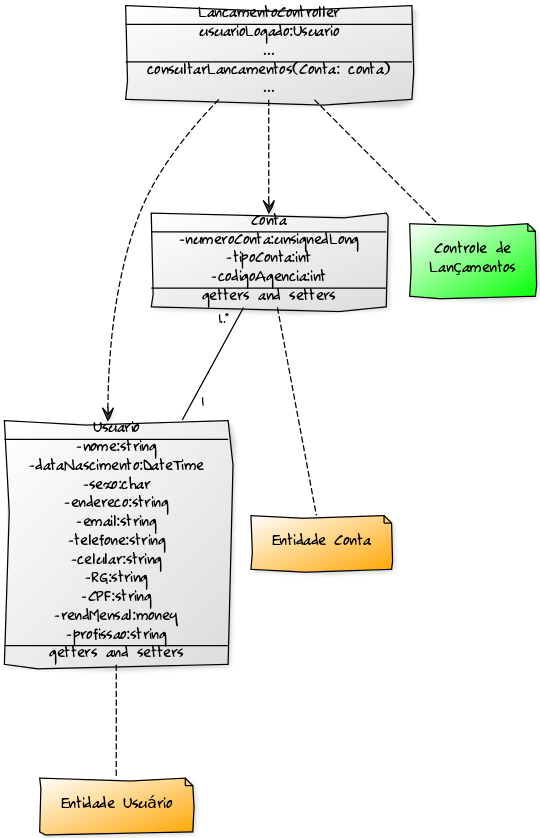
\includegraphics[scale=0.5]{diagramas/diagrama-de-classe/imagens/acompanharLancamentos.png}
     \caption{Diagrama de classes para o caso de uso Bloquear cartão}
     \label{ddc:acompanharLancamentos}
\end{figure}

\section{Realizar compra no cartão de crédito}

Este caso de uso tem como função permitir que o usuário consiga realizar uma compra utilizando seu cartão de crédito.
Após realizar a compra no cartão de cédito, o usuário é notificado por SMS, que está sendo descrito na seção \ref{sec:ReceberSMS}.

\subsection{Caso de uso descritivo}

\begin{table}[h]
  \centering
  \begin{tabular}{|p{4cm} | p{10cm} |}
      \hline
      \small{\textbf{Requisitos Não Funcionais Associados}}	&	Tempo de validação e segurança	\\ \hline
      \small{\textbf{Pré-condição}}	&	O usuário deve ser cliente do banco, possuir uma conta ativa e possuir saldo suficiente na fatura para realizar a compra	\\ \hline
      \small{\textbf{Pós-condição}}	&	A compra é realizada com sucesso e o valor da fatura é acrescido do valor da compra	\\ \hline
    \end{tabular}
 \captionof{table}{Condições para o caso de uso Realizar compra no cartão de crédito}
\end{table}

\textbf{Fluxo de eventos principal:}

\begin{enumerate}
  \item O usuário visita um site de compras e realiza uma compra via cartão de crédito.
  \item O usuário informa os dados do cartão de crédito e permite a cobrança.
  \item O sistema do site de compras envia os dados para o sistema de integração do banco.
  \item O sistema do banco valida os dados.
  \item O sistema verifica se o cliente possui saldo suficiente na sua fatura para realizar a compra.
  \item O sistema concede a cobrança, aumentando assim o valor de sua fatura atual.
  \item O sistema bancário retorna uma resposta de sucesso para o site de compras.
\end{enumerate}

\textbf{Fluxos secundários:}

\begin{itemize}
  \item \textbf{Fluxo secundário – Realizar compra com cartão físico}

  No passo 1, 2 e 3 do fluxo de eventos principal:
  \subitem O usuário vai até uma loja e realiza uma compra com o modo de pagamento cartão de crédito.
  \subitem O usuário insere seu cartão na máquina leitora de cartões e digita sua senha.
  \subitem A máquina leitora envia os dados para o sistema de integração do banco.

  Após o passo 8 do fluxo de eventos principal:
  \subitem A máquina leitora, ao receber a resposta de sucesso exibe a mensagem sucesso ao operador e imprimindo o comprovante.
\end{itemize}

\subsection{Diagrama de caso de uso}

O diagrama para o caso de uso Realizar compra no cartão de crédito pode ser visualizado na Figura \ref{cdu:compraCartaoCredito}.

\begin{figure}[!htb]
     \centering
     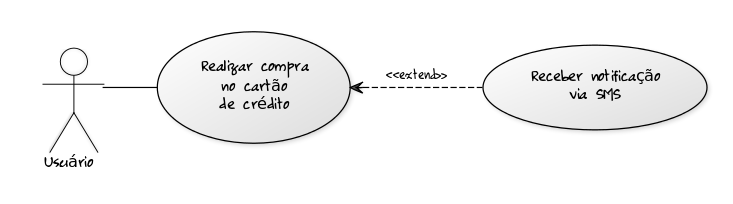
\includegraphics[scale=0.6]{diagramas/caso-de-uso/imagens/realizarCompraCartao.png}
     \caption{Caso de uso Realizar compra no cartão de crédito}
     \label{cdu:compraCartaoCredito}
\end{figure}

\subsection{Diagrama de classes para o caso de uso}

O diagrama de classes para o caso de uso Realizar compra no cartão de crédito pode ser visualizado na Figura \ref{ddc:compraCartao}.

\begin{figure}[!htb]
     \centering
     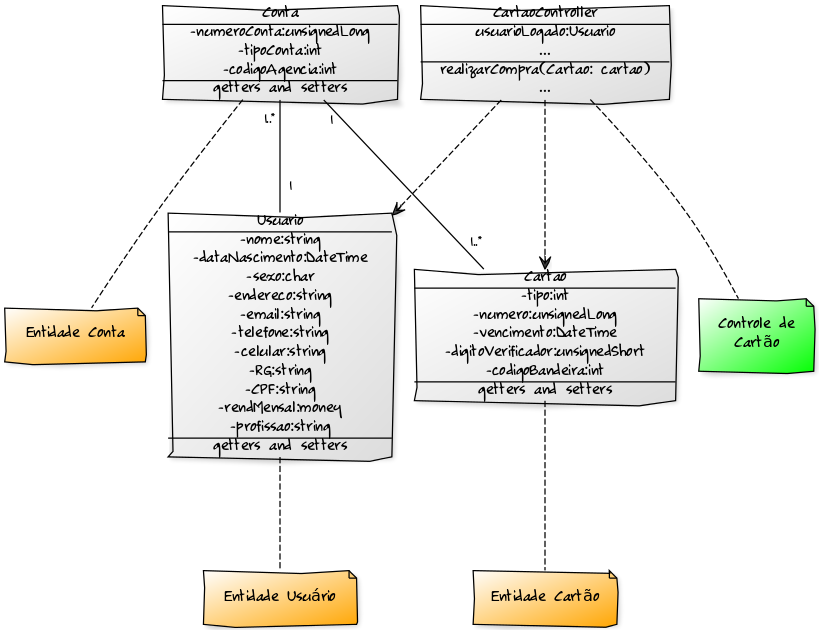
\includegraphics[scale=0.5]{diagramas/diagrama-de-classe/imagens/compraCartao.png}
     \caption{Diagrama de classes para o caso de uso Realizar compra no cartão de crédito}
     \label{ddc:compraCartao}
\end{figure}

\section{Bloquear cartão}

Este caso de uso tem como função permitir que o usuário consiga bloquear o cartão associado a sua conta.

\subsection{Caso de uso descritivo}

\begin{table}[h]
  \centering
  \begin{tabular}{|p{4cm} | p{10cm} |}
      \hline
      \small{\textbf{Requisitos Não Funcionais Associados}}	&	Tempo de acesso, segurança, interface amigável e acessível	\\ \hline
      \small{\textbf{Pré-condição}}	&	O usuário deve ser cliente do banco e deve possuir uma conta ativa	\\ \hline
      \small{\textbf{Pós-condição}}	&	O usuário terá o cartão bloqueado e não poderá utilizá-lo para movimentações bancárias	\\ \hline
    \end{tabular}
 \captionof{table}{Condições para o caso de uso Bloquear cartão}
\end{table}

\textbf{Fluxo de eventos principal:}

\begin{enumerate}
  \item O usuário acessa o sistema utilizando suas credenciais.
  \item O sistema realiza a validação dos dados informados.
  \item O usuário seleciona a opção ``Cartões''.
  \item O sistema exibe opções de cartões referentes a conta.
  \item O usuário seleciona o cartão desejado.
  \item O sistema exibe as opções disponíveis para o cartão selecionado.
  \item O usuário seleciona a opção ``Bloquear cartão''.
  \item O sistema solicita as credenciais do usuário para confirmação do bloqueio do cartão.
  \item O usuário insere as credenciais.
  \item O sistema realiza a validação dos dados informados.
  \item O sistema retorna uma mensagem informando que o cartão foi bloqueado.
\end{enumerate}

\subsection{Diagrama de caso de uso}

O diagrama para o caso de uso Bloquear cartão pode ser visualizado na Figura \ref{cdu:bloquearCartao}.

\begin{figure}[!htb]
     \centering
     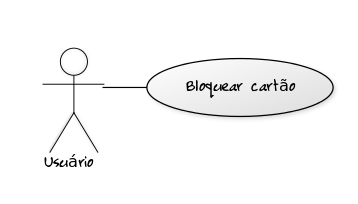
\includegraphics[scale=0.6]{diagramas/caso-de-uso/imagens/bloquearCartao.png}
     \caption{Caso de uso Bloquear cartão}
     \label{cdu:bloquearCartao}
\end{figure}

\subsection{Diagrama de classes para o caso de uso}

O diagrama de classes para o caso de uso Bloquear cartão pode ser visualizado na Figura \ref{ddc:bloquearCartao}.

\begin{figure}[!htb]
     \centering
     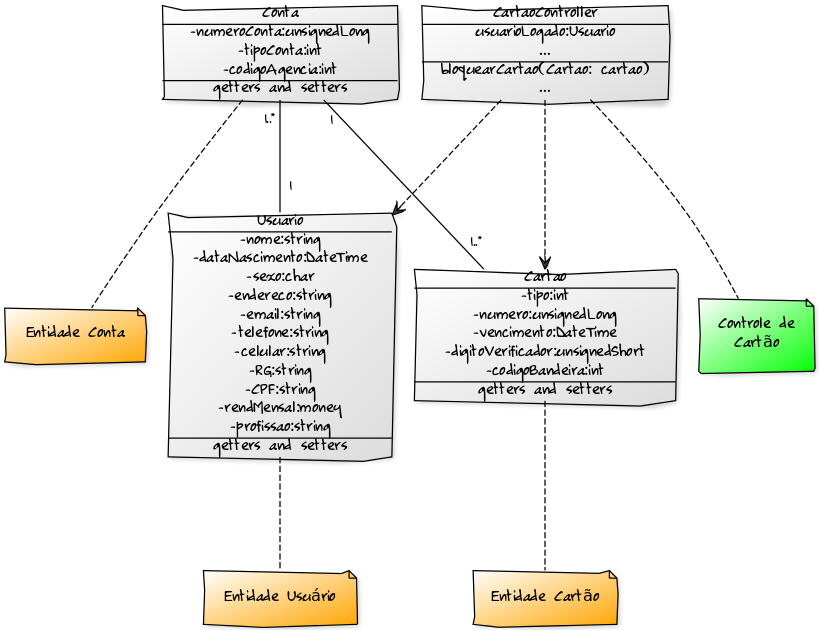
\includegraphics[scale=0.5]{diagramas/diagrama-de-classe/imagens/bloquearCartao.png}
     \caption{Diagrama de classes para o caso de uso Bloquear cartão}
     \label{ddc:bloquearCartao}
\end{figure}

\section{Efetuar saque}

Este caso de uso tem como função permitir que o usuário efetue um saque com ou sem cartão em caixas 24 horas.

\subsection{Caso de uso descritivo}

\begin{table}[h]
  \centering
  \begin{tabular}{|p{4cm} | p{10cm} |}
      \hline
      \small{\textbf{Requisitos Não Funcionais Associados}}	& Tempo de acesso, segurança, interface amigável e acessível	\\ \hline
      \small{\textbf{Pré-condição}}	&	O usuário deve ser cliente do banco, possuir uma conta ativa e ter um saldo mínimo para saque	\\ \hline
      \small{\textbf{Pós-condição}}	&	O saldo da conta do usuário será decrescido do valor do saque e o usuário terá o saque efetuado	\\ \hline
    \end{tabular}
 \captionof{table}{Condições para o caso de uso Efetuar saque}
\end{table}

\textbf{Fluxo de eventos principal:}

\begin{enumerate}
  \item O usuário acessa o sistema utilizando suas credenciais.
  \item O sistema realiza a validação dos dados informados.
  \item O usuário seleciona a opção ``Saque''.
  \item O sistema exibe um campo para que o usuário possa inserir o valor do saque a ser realizado.
  \item O usuário insere o valor desejado.
  \item O sistema solicita ao usuário a confirmação de alguns dados.
  \item O sistema realiza a validação dos dados.
  \item O sistema realiza uma consulta no saldo do usuário para saber se o valor do saque é menor ou igual ao valor total do saldo disponível na conta do usuário.
    \subitem Se o usuário inserir um valor maior do que o saldo total da conta, a máquina de fachada exibe a mensagem ``Saldo insuficiente'' e solicita ao usuário que digite outro valor.
    \subitem Se o usuário possuir saldo suficiente, a máquina de fachada exibe a mensagem ``Aguarde, contando cédulas''.
  \item O sistema exibe a mensagem ``Retire seu dinheiro''.
  \item O usuário retira o dinheiro e encerra a operação.
\end{enumerate}

\textbf{Fluxos secundários:}

\begin{itemize}
  \item \textbf{Fluxo secundário – Efetuar saque utilizando biometria}

  No passo 1 do fluxo de eventos principal:
  \subitem O sistema exibirá uma mensagem informando ao usuário para utilizar a biometria.

  \item \textbf{Fluxo secundário – Efetuar saque sem cartão}
  Pré-condição: Ter habilitado o saque sem cartão em sua conta.

  No passo 1 do fluxo de eventos principal:
  \subitem O usuário informa os dados pessoais solicitados para validação.

\end{itemize}

\subsection{Diagrama de caso de uso}

O diagrama para o caso de uso Efetuar Saque pode ser visualizado na Figura \ref{cdu:efetuarSaque}.

\begin{figure}[!htb]
     \centering
     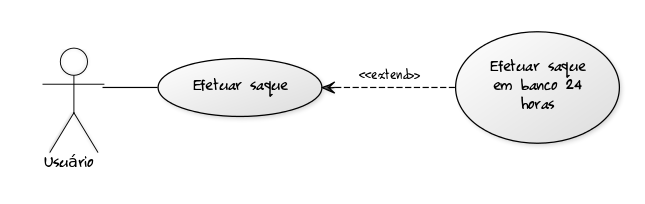
\includegraphics[scale=0.6]{diagramas/caso-de-uso/imagens/efetuarSaque.png}
     \caption{Caso de uso Efetuar saque}
     \label{cdu:efetuarSaque}
\end{figure}

\subsection{Diagrama de classes para o caso de uso}

\section{Receber notificações via SMS}
\label{sec:ReceberSMS}

Este caso de uso tem como função notificar o usuário sobre movimentações feitas em sua conta através de SMS.

\subsection{Caso de uso descritivo}

\begin{table}[h]
  \centering
  \begin{tabular}{|p{4cm} | p{10cm} |}
      \hline
      \small{\textbf{Requisitos Não Funcionais Associados}}	& Tempo de envio, segurança	\\ \hline
      \small{\textbf{Pré-condição}}	&	O usuário deve efetuar alguma movimentação em sua conta e deve ter habilitada a notificação via SMS	\\ \hline
      \small{\textbf{Pós-condição}}	&	O usuário será notificado da movimentação feita em sua conta	\\ \hline
    \end{tabular}
 \captionof{table}{Condições para o caso de uso Receber notificações via SMS}
\end{table}

\textbf{Fluxo de eventos principal:}

\begin{enumerate}
  \item O usuário realiza alguma movimentação em sua conta.
  \item O sistema detecta que houve uma movimentação na conta do cliente.
  \item O sistema envia um SMS informando sobre a movimentação realizada na conta do cliente.
\end{enumerate}

\subsection{Diagrama de caso de uso}

O diagrama para o caso de uso Efetuar saque pode ser visualizado na Figura \ref{cdu:efetuarSaque}.

\begin{figure}[!htb]
     \centering
     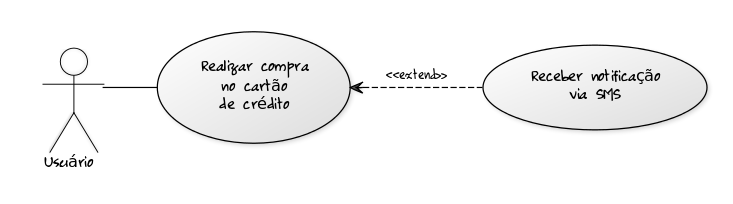
\includegraphics[scale=0.6]{diagramas/caso-de-uso/imagens/receberNotificacaoSms.png}
     \caption{Caso de uso Efetuar saque}
     \label{cdu:efetuarSaque}
\end{figure}

\subsection{Diagrama de classes para o caso de uso}

\section{Usar programa de milhas}

Este caso de uso tem como função permitir que o usuário utilize o programa de milhas para resgatar prêmios.

\subsection{Caso de uso descritivo}

\begin{table}[h]
  \centering
  \begin{tabular}{|p{4cm} | p{10cm} |}
      \hline
      \small{\textbf{Requisitos Não Funcionais Associados}}	& Segurança, interface amigável e acessível, sistema de entregas ligado aos correios	\\ \hline
      \small{\textbf{Pré-condição}}	&	O usuário deve estar realizando o cartão na função crédito continuamente	\\ \hline
      \small{\textbf{Pós-condição}}	&	O usuário receberá o prêmio selecionado tendo seu saldo de milhas decrescido do valor do prêmio	\\ \hline
    \end{tabular}
 \captionof{table}{Condições para o caso de uso Usar programa de milhas}
\end{table}

\textbf{Fluxo de eventos principal:}

\begin{enumerate}
  \item O usuário acessa o sistema utilizando suas credenciais.
  \item O sistema realiza a validação dos dados informados.
  \item O usuário seleciona a opção ``Utilizar programa de milhas''.
  \item O sistema exibe as opções de prêmios que o usuário pode resgatar com as milhas acumuladas.
  \item O usuário seleciona o prêmio desejado.
  \item O sistema verifica se o cliente possui milhas suficientes para resgatar o prêmio selecionado.
  \item Tendo validado, o sistema decresce o valor referente ao prêmio selecionado do saldo de milhas do cliente e viabiliza o resgate.
  \item Após a viabilização, o sistema de envios é informado que deve enviar o prêmio selecionado para o endereço do cliente.
  \item O sistema informa que o prêmio está a caminho do endereço do usuário.
\end{enumerate}

\subsection{Diagrama de caso de uso}

O diagrama para o caso de uso Usar programa de milhas pode ser visualizado na Figura \ref{cdu:programaMilhas}.

\begin{figure}[!htb]
     \centering
     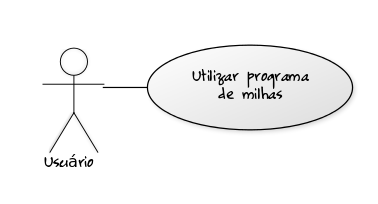
\includegraphics[scale=0.6]{diagramas/caso-de-uso/imagens/utilizarProgramaMilhas.png}
     \caption{Caso de uso Usar programa de milhas}
     \label{cdu:programaMilhas}
\end{figure}

\subsection{Diagrama de classes para o caso de uso}
